\documentclass[a4paper,11pt]{article}

\usepackage[utf8]{inputenc}
\usepackage[english]{babel}
\usepackage{amsfonts,amsmath,amssymb,bbold,dsfont}
\usepackage{calrsfs}
\usepackage[lined,boxed, ruled,vlined, french]{algorithm2e}
\usepackage{multirow}
\usepackage{mathtools,mathptmx}
\usepackage{empheq}
\usepackage{enumerate}
\usepackage{makecell}
\usepackage{tabularx}
\newcommand{\comment}[1]{}
\usepackage{hyperref}

% \usepackage[margin=1in,bindingoffset=15.5mm,heightrounded]{geometry}
% \usepackage{indentfirst}
\usepackage{geometry}

%% for images print/graphiques :
\usepackage{svg}
\usepackage{tikz}
\usetikzlibrary{tikzmark,calc,arrows,shapes,decorations.pathreplacing}
\tikzset{every picture/.style={remember picture}}
\usepackage{accents}
\usepackage{graphicx}
\usepackage{subcaption}

\newcommand\myubar[1]{\underaccent{\bar}{#1}}

%% text color 
\definecolor{ao(english)}{rgb}{0.0, 0.5, 0.0}

%% bibliographie :
% \usepackage{natbib}
% \usepackage[style=authoryear]{biblatex}
% \AtBeginBibliography{\scriptsize}


%% mes shortcuts
\newcommand{\aaa}{\alpha}
\newcommand{\bb}{\beta}


% \usepackage{iflang}
% \usepackage{enumitem}
% \setlist[itemize, 1]{label = \IfLanguageName{french}{\textendash}{\textbullet}}

%%%% mise en page : 
\pagestyle{plain} \setlength{\textwidth}{17,6cm}
\setlength{\textheight}{25cm} \setlength{\topmargin}{-2cm}
\setlength{\oddsidemargin}{-0.9cm}
\setlength{\evensidemargin}{+0.9cm}

%%%%%%%%%%%%%%%%%%%%%%%%%%%%%%%%%%%%%%%%%%%%%%%%%%%%%%%%%%%%%%%%%%%%%%%%%%%%

\title{Projet 5 : Catégorisez automatiquement des questions}
\author{Claire Gayral}
\date{Août 2021}

%%%%%%%%%%%%%%%%%%%%%%%%%%%%%%%%%%%%%%%%%%%%%%%%%%%%%%%%%%%%%%%%%%%%%%%
%%%%%%%%%%%%%%%%%%%%%%%%%%%%%%%%%%%%%%%%%%%%%%%%%%%%%%%%%%%%%%%%%%%%%%
\begin{document}
\maketitle
%%%%%%%%%%%%%%%%%%%%%%%%%%%%%%%%%%%%%%%%%%%%%%%%%%%%%%%%%%%%%%%%%%%%%%%
\tableofcontents
\newpage
%%%%%%%%%%%%%%%%%%%%%%%%%%%%%%%%%%%%%%%%%%%%%%%%%%%%%%%%%%%%%%%%%%%%%%%
\section*{Introduction}
Stack Overflow, ce site utilisé presque quodiennement par la plupart des personnes amenées à écrire du code, n'est pas si simple à utiliser pour les novices d'un outil informatique, puisqu'il s'appuie sur un système de tags, issus d'une sémantique propre. L'idée du projet 5 de la formation "Ingénieur Machine Learning" d'OpenClassroom est justement de proposer une solution de suggestion de tags à partir de la question. Du nettoyage des données aux différents modèles d'apprentissage, en passant par les méthodes de réduction propres au text-mining, ce document présente le travail effectué pour répondre à cette problématique.

\section{Analyse exploratoire}
La première étape, quelque soit le modèle, va être de nettoyer les posts, et d'en extraire les mots pertinents. Pour l'approche supervisée, les tags formeront les classes à prédire, et pour l'approche non supervisée, les labels permettront de comparer les projections (les mots les plus importants pour chaque topics) et les tags proposés dans le poste. 


\subsection{Choix des tags}
Pour la modélisation supervisée, il est nécessaire de disposer des tags de sortie. Cependant, dans les posts de Stack Overflow, il y a plusieurs tags pour chaque sujet. Comme la classification multi-classe peut vite s'avérer complexe (problème de dimension, interprétabilité), il faut réduire la complexité des tags en entrée. 

Un premier pré-traitement permet de limiter la perte d'information. Par exemple, les tags faisant références à différentes versions du même langage sont homogénéisés afin de limiter la perte d'information. Par ailleurs, les tags qui n'apparaissent que dans un post sont trop peu informatif, et ne seront pas conservés. 
\subsubsection*{Choix d'une variable de sortie univariée}
Pour une classification univariée, le choix le plus simple est de prendre le tag qui apparait le plus souvent. C'est ainsi que la classification supervisée univariée fera référence au tags "csharp"
\begin{center}
   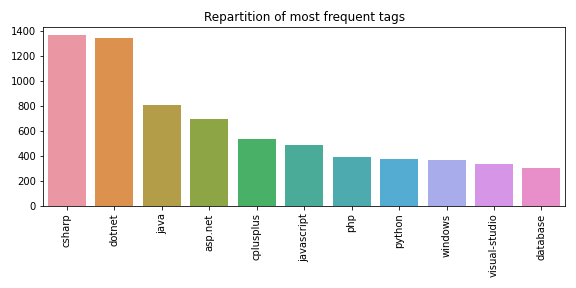
\includegraphics[width=0.8\linewidth]{figures/most_freq_tags.png}
\end{center}

\subsubsection*{Réduction de dimension}
Une première projection sur des axes choisis (NMF, PCA ou SVD) permet de vérifier s'il existe une structure algébrique qui permet de caractériserr la répartition des tags dans les posts. Ces méthodes de projection permettraient de contruire des méta-tags comme pondération sur les tags à partir des composantes. Cependant, même avec une régularisation Lasso, chaque dimension est soit très fortement tirée par un ou deux tags, soit avec une composition de beaucoup de tags différents. 

\begin{center}
   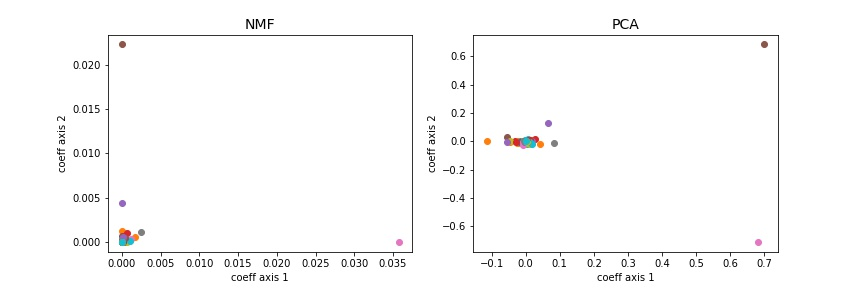
\includegraphics[width=0.8\linewidth]{figures/tags_NMF_PCA_coeffs12.jpg}
\end{center}

Ensuite, une réduction de dimension par regroupement en communauté permet de regrouper certains tags qui apparaissent dans plusieurs posts. 

Un clustering hierarchique est alors plus pertinente : cette approche permet de choisir à postériori où tronquer l'arbre, pour obtenir suffisament peu de cluster, et garder des clusters qui ont un sens, et qui sont suffisamment représentés dans les données pour apprendre le lien avec le texte des posts. 

\begin{center}
   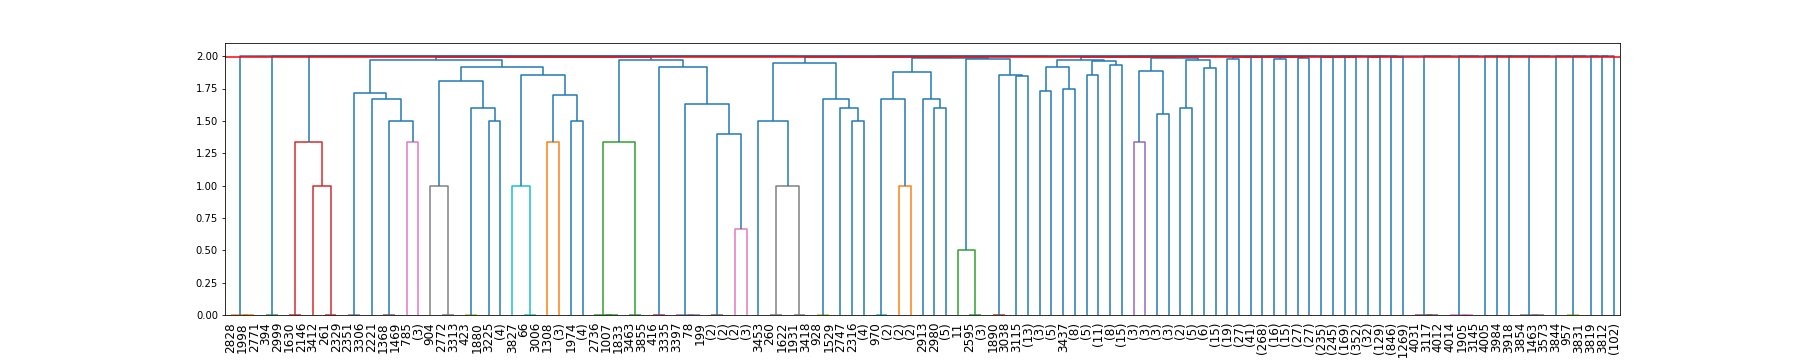
\includegraphics[width=\linewidth]{figures/hierarchical_clustering.png}
\end{center}
Par exemple, le cluster numéro 46 de la classification donnée par le tronquage de la ligne rouge (à 1.99) regroupe les termes suivant, faisant tous référence à la création de site web avec python : \\
{\small \centering \texttt{3des, active-directory, active-directory-group, activex, adam, android-emulator, apache2, app-config, asp.net-membership, assert, atl, authentication, authkit, authorization, azman, bho,  bouncycastle, center, certificate, code-snippets, cracking, crash,  crash-reports, credentials, cryptoapi, cryptographicexception,  cryptography, delegation, diffie-hellman, directoryservices,  distribution-list, distro, django, django-authentication,  django-models, django-templates, django-urls, django-users, dojo,  e-commerce, encryption, fastcgi, fcgid, firebug, firephp,  forms-authentication, gnu, gnupg, greasemonkey, http-authentication,  intellisense, internet-explorer, intranet, javascript-debugger,  jcifs, kerberos, key-events, key-storage, knowledge-management,  ldap, ldap-query, leaderboard, limits, login, logrotate,  mediawiki-extensions, membership, metabase, mode, ntlm, passphrase, passwords, payment, pci-dss, pdc, penetration-testing, pgo, pgp,  phpbb, precompiled-headers, protected, pylons, query-optimization,  ram-scraping, rest-security, roles, sam, sco-unix, security,  security-zone, segmentation-fault, shopping-cart, spn, ssl, sspi,  stack-trace, svn-administraton, symmetric-key, sysdba,  template-engine, text-align, tool-rec, web-config, wildcard-mapping,  x509, gplusplus}}\\

Du clustering, j'extrait 12 clusters que mes connaissances informatiques permettaient d'identifier : \\
{\small \centering \texttt{ linux, language, microsoft, micro\_service, create\_website, python\_website, ruby, tests, python, computer\_architecture, multimedia, object\_oriented }}
\begin{center}
   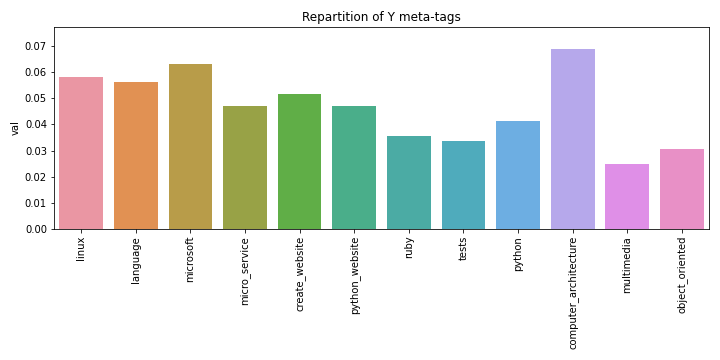
\includegraphics[width=\linewidth]{figures/Y_distribution.png}
\end{center}

% Et de façon plus globale, les méta-tags sont répartis dans les postes comme suit : 
% \begin{center}
%   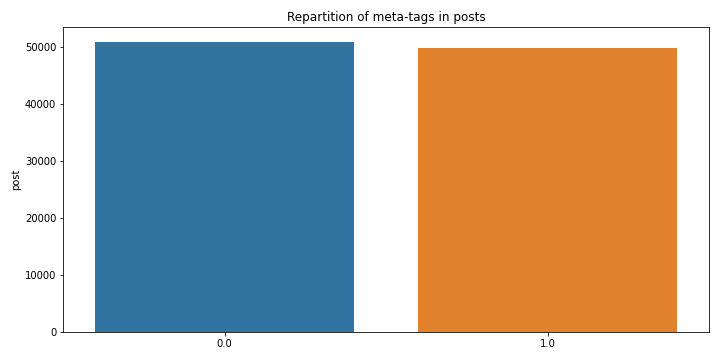
\includegraphics[width=\linewidth]{figures/Y_repartition_in_posts.png}
% \end{center}

% TODO commenter plus ?


\subsection{Prétraitements de textes}

Dans un premier temps, il fallait choisir une façon de représenter les mots, et en extraire leur sémantique. Pour cela, j'ai effectué un prétraitement contenant :\\
% \vspace{0.3cm}

Les différentes étapes sont illustrées sur la phrase suivante :\\
{\small \centering \centering
    \texttt{%How to unload a ByteArray using Actionscript 3?\\
    <p>How do I forcefully unload a <code>ByteArray</code> from memory using ActionScript 3?</p>}
}
\begin{enumerate}
    \item Changement de format et suppression de la ponctuation, filtre pour regrouper les différentes versions des langages de programmation\\
        {\small \centering
        \texttt{%how, to, unload, a, bytearray, using, actionscript, 
        how, do, i, forcefully, unload, a, bytearray, from, memory, using, actionscript'}
        }
    \item Retrait des mots de transition ou très présents (stop words)\\
        {\small \centering
        \texttt{%unload, bytearray, actionscript,
        forcefully, unload, bytearray, memory, actionscript}
        }
    \item Lemmatisation\\
        {\small \centering
        \texttt{%unload, bytearray, actionscript,
        forc, unload, bytearray, memori, actionscript}
        }
\end{enumerate}

Ces traitements permettent de réduire progressivement la dimension des données textuelles, en ne conservant que les informations pertinentes. L'évolution de la répartition des mots peut être suivie par différentes statistiques telles que le nombre d'apparition des mots dans les postes : \\

{\small 
\begin{minipage}{0.48\linewidth}
    1. Répartition des mots dans le corpus original :%avant la suppression des mots de transition :
    \begin{center}
        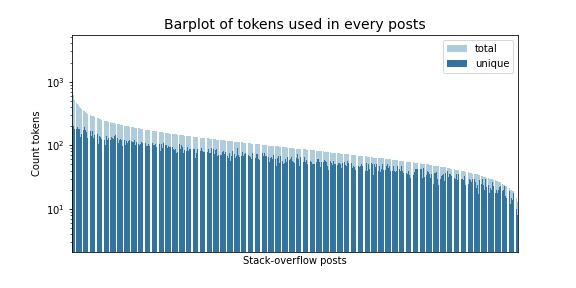
\includegraphics[width=\linewidth]{figures/barplot_tokens1.jpg}
    \end{center}
\end{minipage}
\hfill
\begin{minipage}{0.48\linewidth}
    2. Répartition des mots après les pré-traitements :
    \begin{center}
        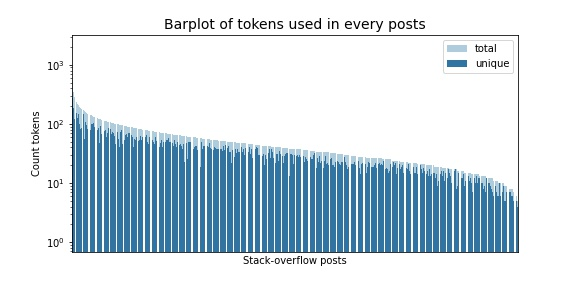
\includegraphics[width=\linewidth]{figures/barplot_tokens3_radical.jpg}
    \end{center}
\end{minipage}
% \hfill
% \begin{minipage}{0.33\linewidth}
%     3. Répartition des mots après la lemmatisation 
%     \begin{center}
%         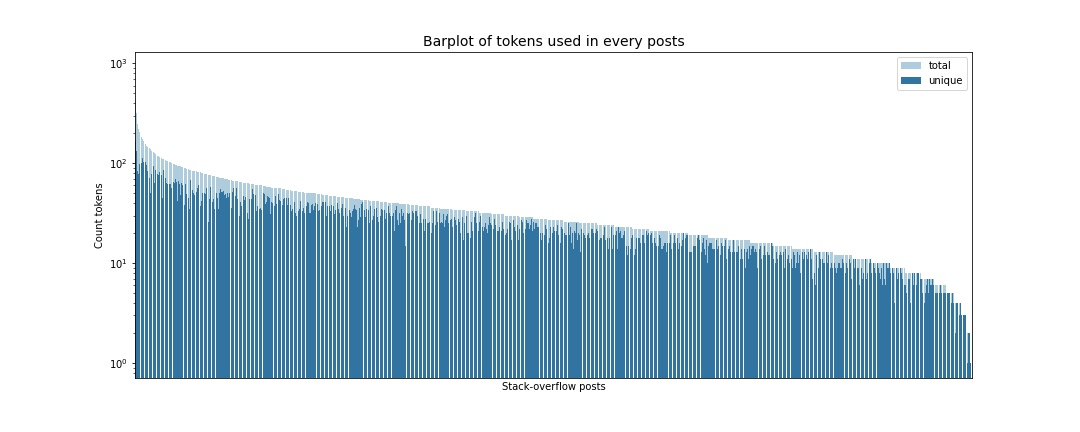
\includegraphics[width=\linewidth]{figures/barplot_tokens4_radical.jpg}
%     \end{center}
% \end{minipage}
}\\

Ces différents prétraitements donnent accès à une liste de pseudo-mots appelés tokens. Ces ensembles de tokens {\color{blue} \href{https://openclassrooms.com/fr/courses/4470541-analysez-vos-donnees-textuelles/4855001-representez-votre-corpus-en-bag-of-words}{peuvent être représentés de différente façon}} selon les modèles statistiques pour lesquellent ils vont être utilisés.
\begin{itemize}
    \item bag of words (BOW) : C'est la représentation naturelle, consistant en une matrice réprésentant le nombre d'occurence de chaque mots dans les différents postes. Commes il y a beaucoup de mots différents et que très peu de mots sont appelés dans chaque postes, cette matrice est très creuse.
    \item tfidf : Une pondération des différents tokens prenant en compte leur rareté
    \item word2vec : D'autres représentations existent et sont plus complexes, s'appuyant sur des modèles de NLP déjà entraînés.
\end{itemize}

Les mots peuvent aussi être représentés graphiquement, notamment à l'aide de nuages de mots comme suit :

\begin{minipage}{0.48\linewidth}
    \begin{center}
       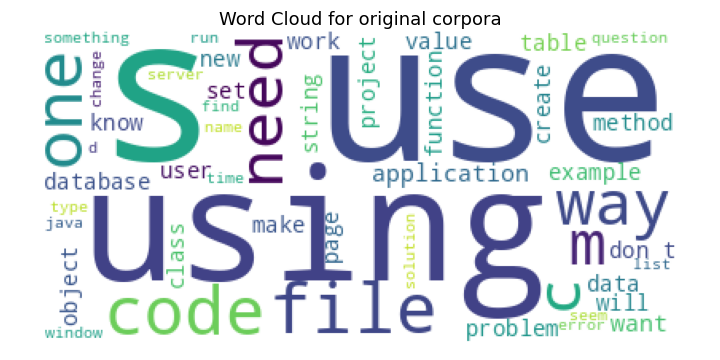
\includegraphics[width=\linewidth]{figures/word_cloud_corpora.png}
    \end{center}
\end{minipage}
\begin{minipage}{0.48\linewidth}
    \begin{center}
       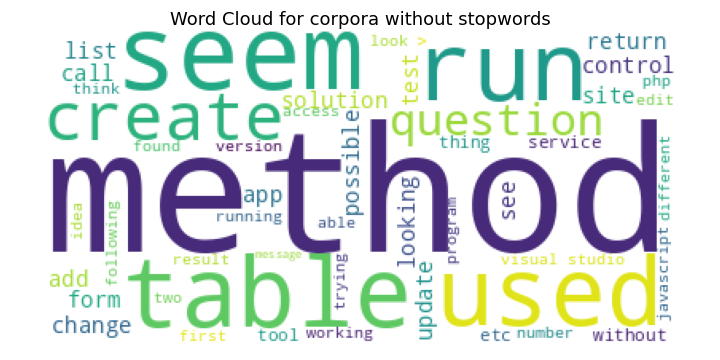
\includegraphics[width=\linewidth]{figures/word_cloud_corpora2.png}
    \end{center}
\end{minipage}

Ces illustrations permettent par exemple de voir l'importance de retirer les mots de liaisons tels que "S" ou "need" ou "one". \\

Le corpus sans stopwords, et lemmatisé servira de données d'entrainement pour la suite. Pour rappel, l'objectif de ce projet est de proposé des tags de façon automatique. Pour cela, deux approches différentes sont utilisées. La première est non supervisée : on cherche des tags sans apriori, c'est-à-dire sans utiliser les tags liés aux publications. A l'inverse, la deuxième approche apprend le lien entre la distribution des tags et la distribution des mots dans les publications.
    
\section{Prédiction de tags}
Nous allons donc proposer et tester différents modèles pour prédire les tags, puis les comparer.

\subsection{Modélisation non supervisée}

Une première approche consiste à projeter la distribution des mots dans des espaces réduits, que l'on appellera "topic". Les phrases alors projetées seront une combinaison de ces topics : plus le poids du topic est grand, plus la phrase est dans ce thème. Comparer les différentes projections, la métrique utilisée est le MSE, c'est-à-dire l'erreur moyenne au carrée entre la table orginale et sa projection dans l'espace réduit. Ce critère, à minimiser, permet dans un premier temps de choisir les meilleurs paramètres pour chaque modèles, puis de choisir le modèle le plus adapté.

\subsubsection*{La NMF}
%% La méthode
Comme pour la projection non supervisée des tags, comme tous les coefficients sont positifs, on peut faire appel à la {\color{blue} \href{https://en.wikipedia.org/wiki/Non-negative_matrix_factorization}{"Non-Negative Matrix Factorization" (NMF)}} pour projeter les tokens dans des espaces sémantiques. Cette méthode de projection est une décomposition de la matrice des mots en BOW. Il s'agit de trouver les variables latentes (topics) qui expliquent au mieux la structure de covariance entre les variables. Contrairement à la PCA, qui maximise la variance dans l'espace projeté, la NNF n'a pas de contrainte d'orthonormalité. \\

%% les données en entrée
Pour cette partie, le pré-traitement du corpus est relancé avec le module de sklearn, afin d'accéder facilement aux features, comme proposé dans {\color{blue} \href{https://scikit-learn.org/stable/auto_examples/applications/plot_topics_extraction_with_nmf_lda.html#sphx-glr-auto-examples-applications-plot-topics-extraction-with-nmf-lda-py}{cet exemple de sklearn}}. \\

%% optimisation des paramètres
Le choix des hyper-paramètres est fait par une pseudo validation croisée. L'ensemble d'entrainement est divisé en différents folds. Le modèle est alors appris sur un sous-ensemble de l'entrainement initial, et validé sur la partie laissée intacte. On ne peut pas vraiment parler de validation croisée car il n'y a pas de sortie visée, la métrique sur l'ensemble de validation ne fait pas référence à une sortie mais à la similitude, mesurée par le MSE, entre la validation et sa projection dans le sous-modèle. 

Ainsi, les paramètres optimaux sont choisis par la lecture des graphiques suivants : 

\begin{center}
    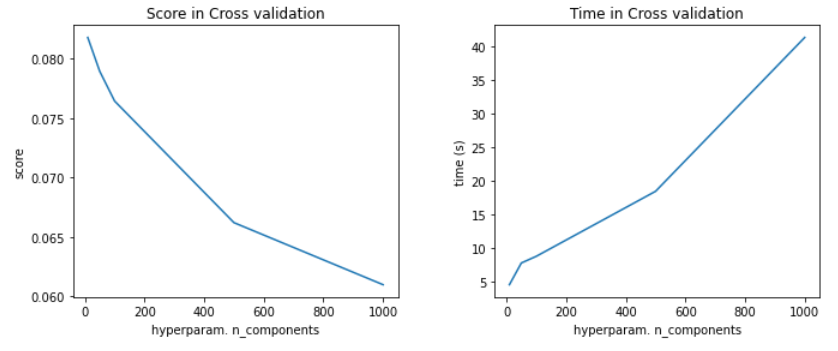
\includegraphics[width=0.8\linewidth]{illustrations/corpus_NMF_set_n_components.png}
    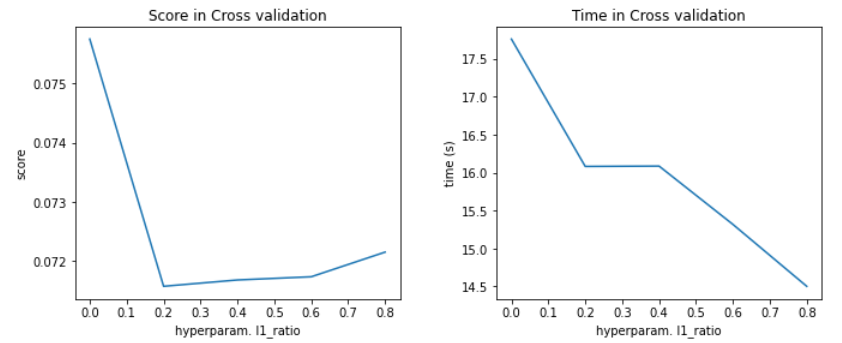
\includegraphics[width=0.8\linewidth]{illustrations/corpus_NMF_set_l1_ratio.png}
\end{center}

Par exemple, pour la NMF sur ce corpus, le meilleur modèles est choisi avec 20 composantes et une régularisation lasso de 0.2. Ces 20 composantes ne sont pas le meilleur paramètre, puisque le score chutte encore après 500 composantes, néansmoins, il devient trop fastidieux d'explorer autant de topics. 


%% évaluation du modèle : 
Bien que pratique à manier, le MSE donne peu d'information quant à la pertinence de la projection. Il est alors intéressant de regarder le poids des principaux mots pour les topics. 

\begin{center}
    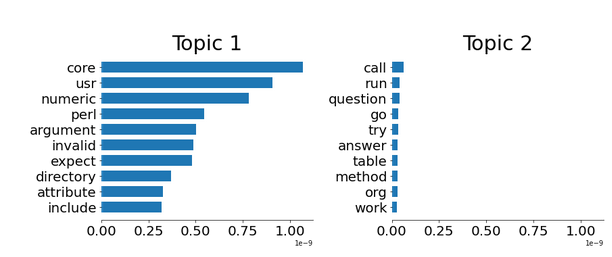
\includegraphics[width=0.8\linewidth]{illustrations/coprus_NMF_topics2.png}
\end{center}


\subsubsection*{La LDA}
Une autre méthode de projection basée sur un modèle génératif, la {\color{blue} \href{https://fr.wikipedia.org/wiki/Allocation_de_Dirichlet_latente}{"Latent Dirichlet Allocation"}} est un modèle bayésien couramment utilisé pour l'extraction de topics. \\


\begin{minipage}{0.5\linewidth}
    Le modèle graphique probabiliste de la LDA est le suivant\\
    Cette figure est issue de {\color{blue} \href{http://www.jmlr.org/papers/volume3/blei03a/blei03a.pdf}{l'article orginale de la LDA}}. Le consulter pour le détail du sens de chaque variable latente.
\end{minipage}
\hfill
\begin{minipage}{0.4\linewidth}
    \begin{center}
       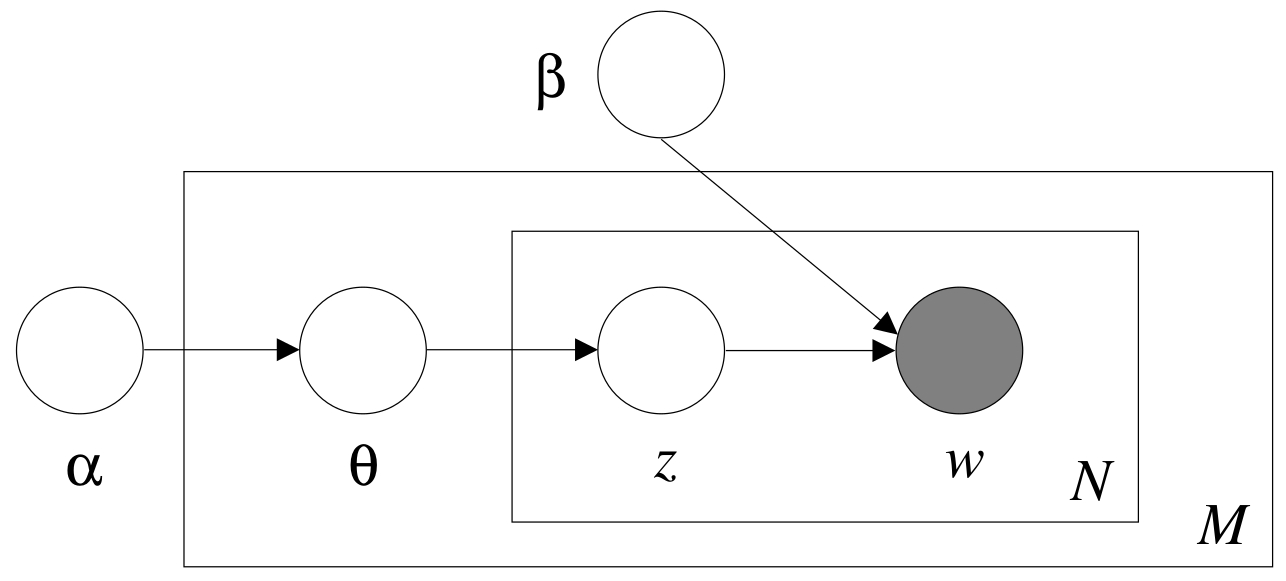
\includegraphics[width=0.8\linewidth]{illustrations/PGM_LDA_original.png}
    \end{center}
\end{minipage}

\vspace{0.2cm}

Avec la même méthodologie que celle présentée pour la NMF, les paramètres du modèle sont fixés à learning\_decay = 0.9, learning\_offset = 100, n\_components = 2000, max\_iter = 5. Bien que ce soit le modèle le plus fidèle aux données, il est fastidieux de trouver un nom pour chaque topics lorsqu'il y en a 2000. Pour aller au bout du projet, j'ai donc réduit le nombre d'axes de projection, à 20 classes, les autres paramètres de la LDA sont adaptés à cette contrainte. Les 20 classes sont alors résumées comme suit : 

\begin{center}
   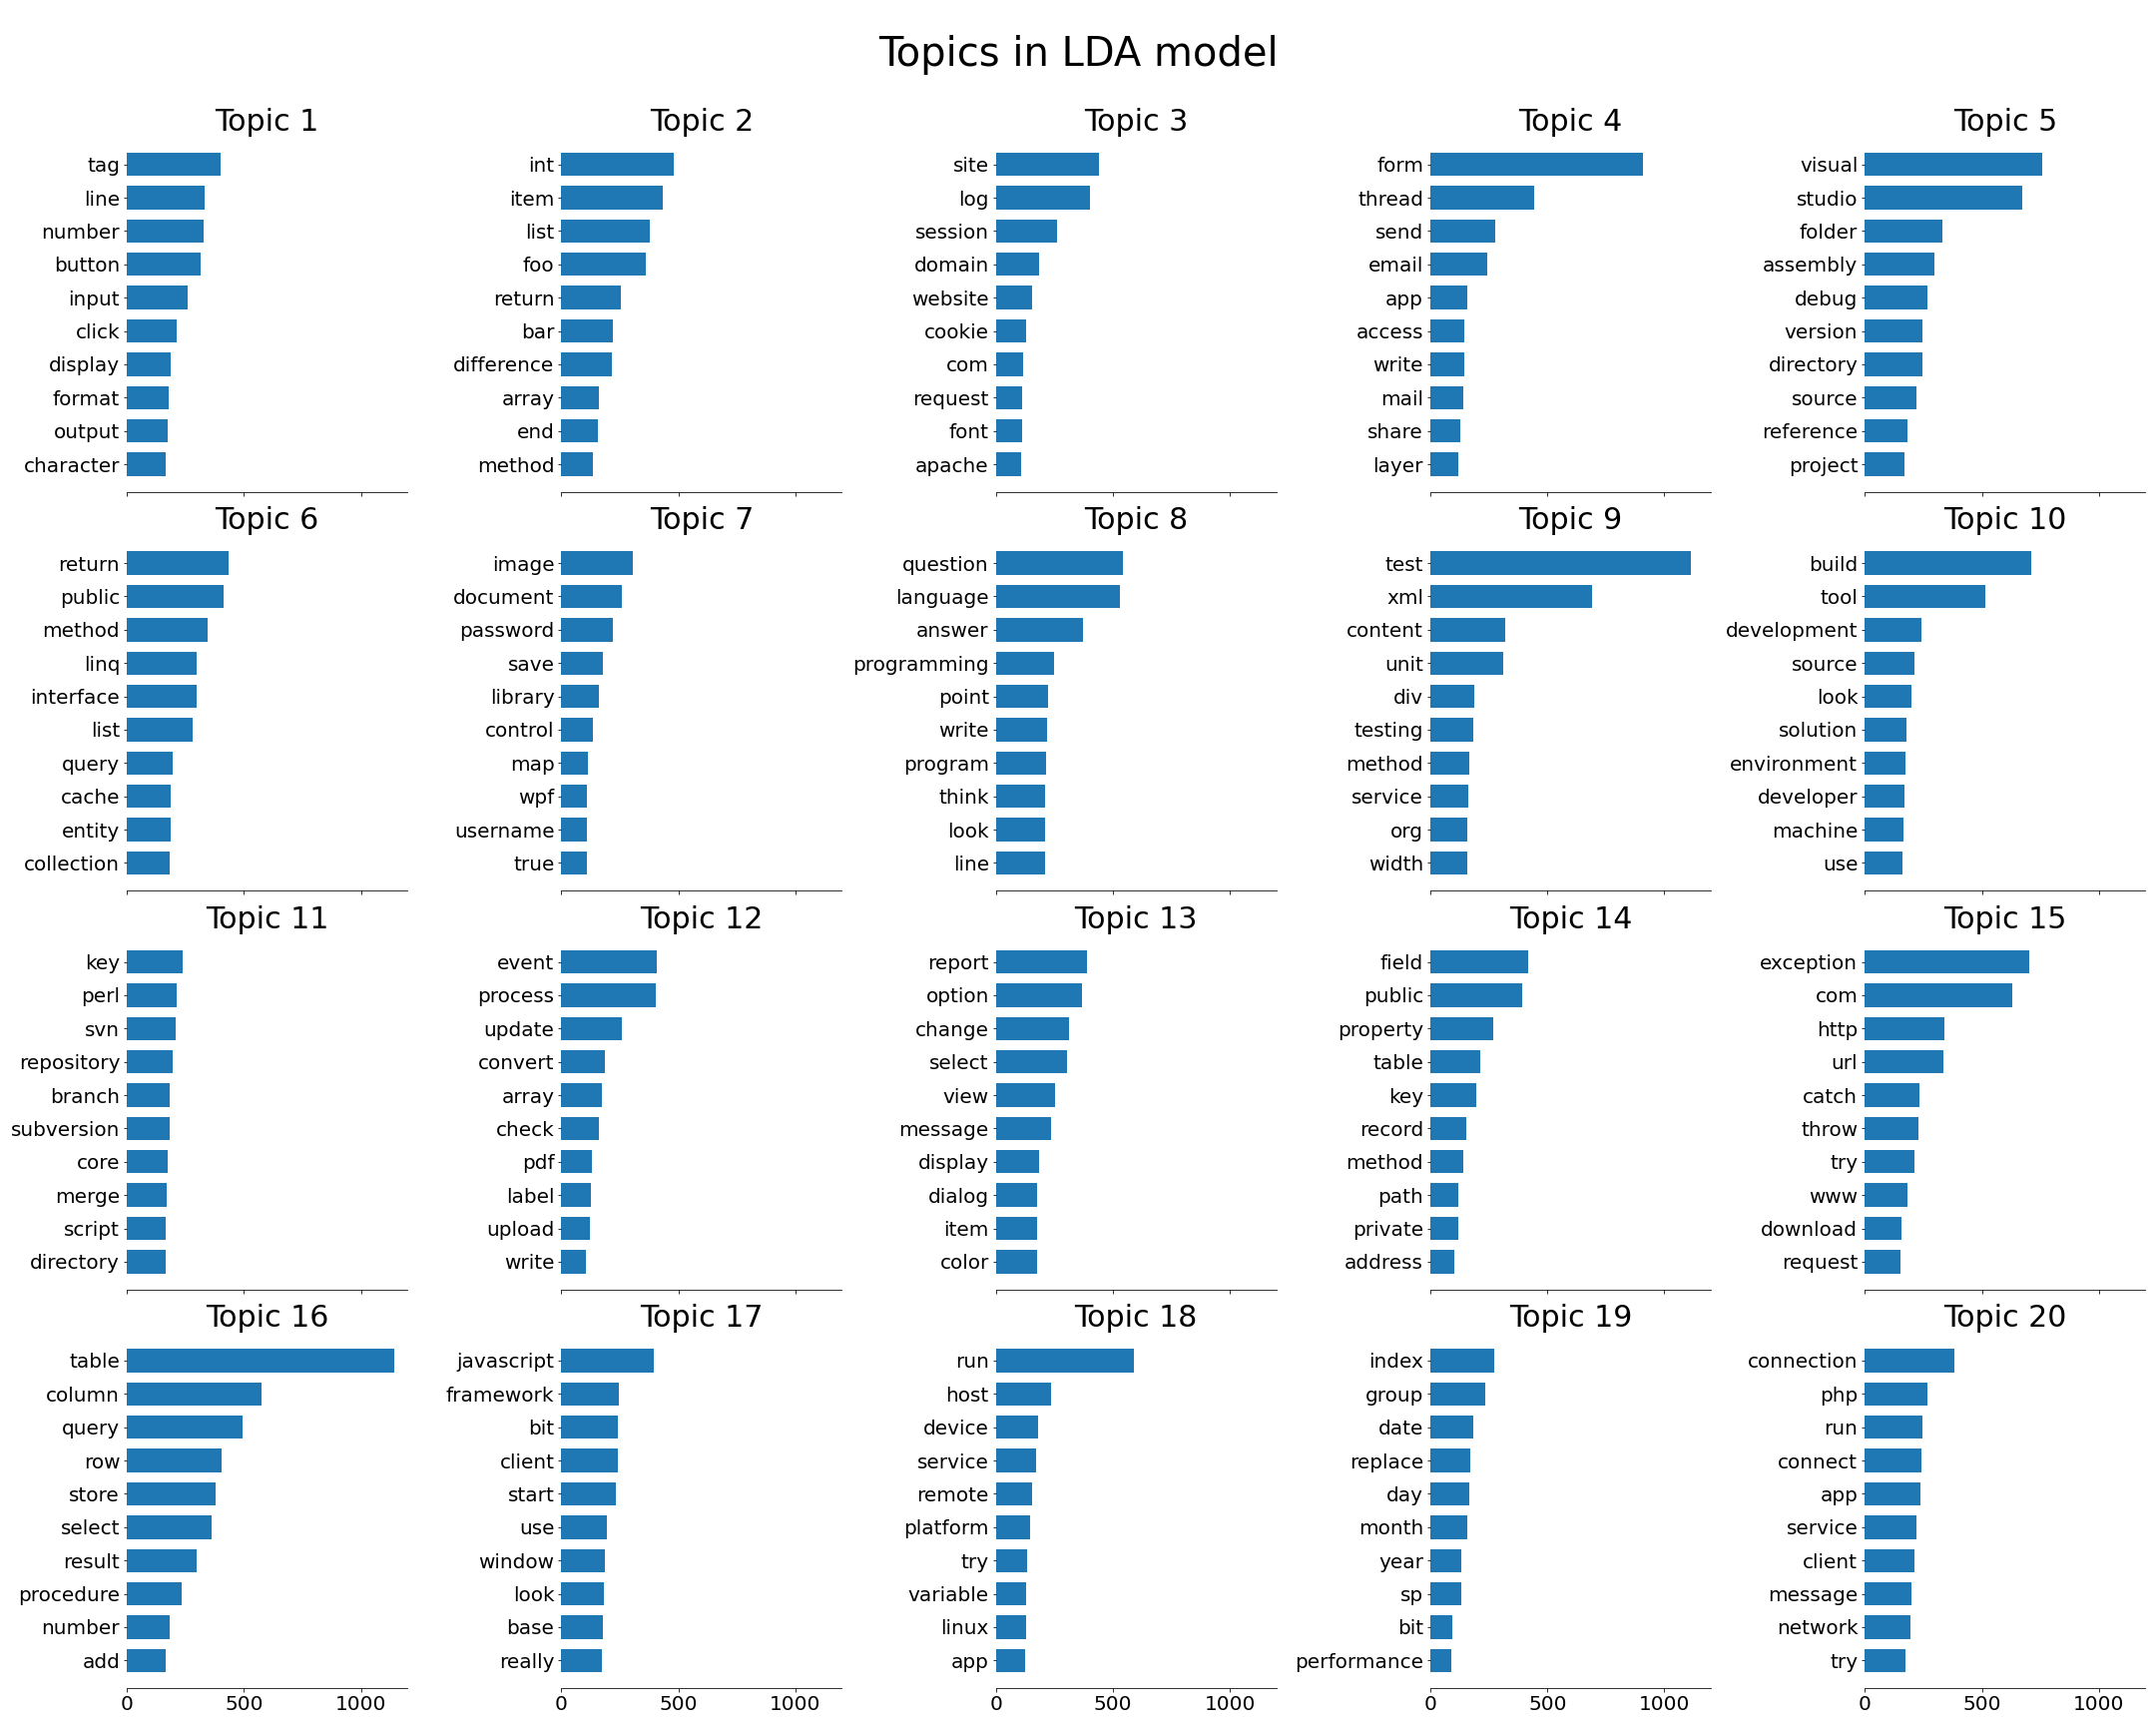
\includegraphics[width=0.9\linewidth]{figures/coprus_LDA_small_topics.png}
\end{center}

Ainsi, la prédiction de tags à partir de cette table implique une labellisation des topics à partir de leur sémantique, comme le topic 1 semble référer à l'UI, le deuxième aux manipulations de base,...

Il est possible d'explorer les différentes sémantiques à l'aide de l'outil de visualisation pyLDAviz, donc l'interface est la suivante :

\begin{center}
   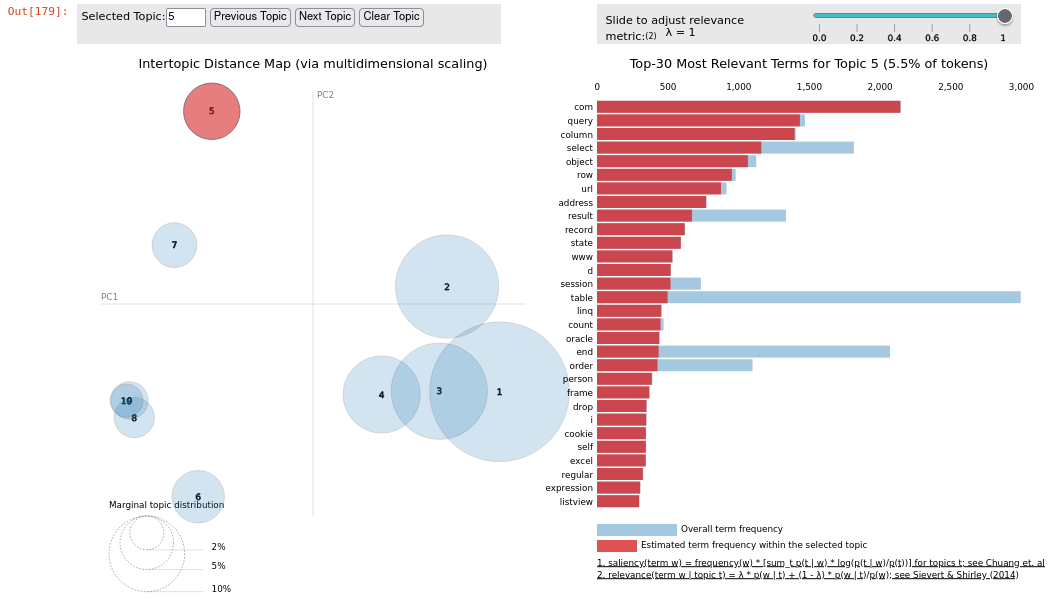
\includegraphics[width=\linewidth]{illustrations/pyLDAviz_topic5_web.png}
\end{center}
La visualisation ne correspond pas au même modèle de LDA que celui proposé dans la décomposition des topics, car le premier modèle est sklearn, le deuxième gensim.


\subsubsection*{Comparaison des modèles sur l'ensemble test}
L'objectif était de prédire les tags les probables pour les publication de l'ensemble de test. On peut au moins prédire les topics pour chaque post, et en constituer un tag. 


\section{Modélisation supervisée}
Ensuite, des modèles supervisés sont entrainés pour apprendre le lien entre la distribution des mots dans les postes, et les tags associés. Un premier travail consiste à apprendre les relations entre la distribution des mots et le tag en question. Un deuxième axe de travail cherche une classification en plusieurs classes, à partir des méta-tags construits dans la première partie. 

\subsection{Présentation des modèles utilisés}

Les 3 modèles suivants sont couramment utilisé pour la classification de texte. 

\subsubsection*{Naive Bayes}
La classique classification de Bayes Naive suppose que les variables sont indépendantes et renversent le théorème de Bayes pour prédire la classe la plus probable conditionnée aux mots observés. Ces classificateurs naïfs {\color{blue} \href{https://mrmint.fr/naive-bayes-classifier}{sont très courants pour la classification de texte}}. 

Ces modèles assez simples n'ont que deux paramètres à fixer. Il s'agit d'une part de la loi de probabilité des mots. Je testerai avec une Bernoulli Negative Binomiale, une Complement Negative Binomiale, et Mutlinomial Negative Binomiale. Le deuxième paramètre, alpha, un paramètre de régularisation 
Pour chaque modèle, le choix du meilleur alpha est fait par validation croisée. 
L'accuracy du meilleur model est de presque $90\percent$ sur l'ensemble de test.


\subsubsection*{Gradient Boosting }

Le Gradient Boosting est une méthode de recherche de minimum pour une perte donnée, pour laquelle la descente de gradient est faite sur plusieurs arbres décisionnels, pour éviter de tomber dans des minima locaux. Ainsi, cette méthode dépend énormément de la métrique choisie. Pour {\color{blue} \href{https://machinelearningmastery.com/metrics-evaluate-machine-learning-algorithms-python/}{la classification binaire}}, on peut par exemple tester la perte logistique, ou exponentielle, l'accuracy ou encore l'AUC. Je resterai basique en comparant les pertes logisitique et exponentielle. \\

\begin{minipage}{0.45\linewidth}
    Perte logistique : 
    $$ a $$
\end{minipage}
\hiff
\vline
\hfill
\begin{minipage}{0.45\linewidth}
    Perte exponentielle : 
    $$ b $$
\end{minipage}\\


\subsubsection*{Random Forest}
Les forêts aléatoires - Randoms Forest en anglais - sont des méthodes de classification pour lesquelles plusieurs arbres décisionnels dits faibles sont calculés, à partir d'un sous-ensemble de l'entrainement. Le modèle de classification final est alors obtenu par un vote à la majorité des classifieurs. 
Comme pour les autres méthodes, les paramètres de ce modèles sont sélectionnés par validation croisée. 

\subsection{Classification binaire}
Dans cette partie, le tag a été choisi comme le tag le plus présent dans les postes, il s'agit du langage "csharp". Les modèles suivants cherchent à produire une classification des données en "fait référence à csharp" et "ne fait pas référence à csharp". Il serait alors possible de produire un classifieur par tag, et garder au final comme prédiction les tags les plus probables pour chaque publication.\\ 

Deux modèles ont été testés pour cette tâche : les modèles Naive Bayes, et le gradient boosting. Pour sélectionner et comparer les modèles, on utilisera l'accuracy, définie comme le quotien entre le nombre de prédiction correcte et le nombre de prédiction totale. Une classification aléatoire aurait alors une accuracy égale à $\frac{1}{2}$.

\subsection{Classifieur multi-classe}
Une classification aléatoire aurait alors une accuracy égale à $\frac{1}{\text{nb de classe}}$



% \section{Choix du modèle et déploiement}
% \subsection{Tests}
% \subsection{Manuel d'utilisation}

\section*{Conclusion}
A améliorer :

\begin{itemize}
    \item Tester l'influence des différents pré-traitements et représentations des mots
    \item D'autres modèles pré-entrainés et sûrement beaucoup plus performants existents. BERT en est un exemple. Cela aurait été intéressant d'explorer cette méthode.

\end{itemize}


Biblio : 
\begin{itemize}
    \item Prétraitements du corpus :
        \begin{itemize}
            \item {\color{blue} \href{http://www.nltk.org/book/}{Une référence tès complète sur le NLP}}
            \item  {\color{blue} \href{https://openclassrooms.com/fr/courses/4470541-analysez-vos-donnees-textuelles/ }{Le cours d'OC sur le traitement des données textuelles}}
            \item Deux bibliothèque principales python : {\color{blue} \href{https://radimrehurek.com/gensim/}{gensim}} et {\color{blue} \href{ https://scikit-learn.org/stable/tutorial/text_analytics/working_with_text_data.html}{scikit-learn}}
        \end{itemize}
    \item Représentation des mots : 
        \begin{itemize}
            \item {\color{blue} \href{https://openclassrooms.com/fr/courses/4470541-analysez-vos-donnees-textuelles/4855001-representez-votre-corpus-en-bag-of-words}{Cours d'OC sur la représentation des mots} }
            \item {\color{blue} \href{https://www.kaggle.com/c/word2vec-nlp-tutorial#part-1-for-beginners-bag-of-words}{Word 2 vect} }
        \end{itemize}
        
    \item Extraction de mots-clé (non supervisé) - généralités :
        \begin{itemize}
            \item {\color{blue} \href{https://jios.foi.hr/index.php/jios/article/view/938/724}{Article overview}}
            \item {\color{blue} \href{https://www.irit.fr/IRIS-site/images/seminairs/Thonet2016.pdf}{Slide de présentation séminaire sur "Topic Models" Thibaut THONET}}
        \end{itemize}
    \item NMF :
        \begin{itemize}
            \item {\color{blue} \href{https://en.wikipedia.org/wiki/Non-negative_matrix_factorization}{La page wikipedia}}
            \item {\color{blue} \href{https://openclassrooms.com/fr/courses/4379436-explorez-vos-donnees-avec-des-algorithmes-non-supervises/4379511-cherchez-les-variables-latentes-qui-expliquent-vos-donnees}{Le cours d'OpenClassRooms sur les méthodes non supervisées}}
            \item {\color{blue} \href{https://scikit-learn.org/stable/modules/generated/sklearn.decomposition.NMF.html}{La doc de scikit-learn}} et {\color{blue}\href{https://scikit-learn.org/stable/auto_examples/applications/plot_topics_extraction_with_nmf_lda.html#sphx-glr-auto-examples-applications-plot-topics-extraction-with-nmf-lda-py}{un exemple d'utilisation pour l'extraction de topics}}
        \end{itemize}
    \item LDA : 
        \begin{itemize}
            \item {\color{blue} \href{https://fr.wikipedia.org/wiki/Allocation_de_Dirichlet_latente}{La page wikipedia}}
            \item {\color{blue} \href{https://www.analyticsvidhya.com/blog/2021/06/part-2-topic-modeling-and-latent-dirichlet-allocation-lda-using-gensim-and-sklearn/}{Un article sur l'extraction de topic avec la LDA}}, un {\color{blue} \href{https://towardsdatascience.com/light-on-math-machine-learning-intuitive-guide-to-latent-dirichlet-allocation-437c81220158}{autre article}}
            \item {\color{blue} \href{La page du code de l'article original}{https://github.com/blei-lab/onlineldavb}}
        \end{itemize}
    \item Naive Bayes:
        \begin{itemize}
            \item {\color{blue} \href{https://www.analyticsvidhya.com/blog/2017/09/naive-bayes-explained/}{Une explication illustrée}}
            \item {\color{blue} \href{https://monkeylearn.com/blog/practical-explanation-naive-bayes-classifier/}{Un article similaire - des idées à la programmation, sur la prédiction de lien sémantique}}
            \item {\color{blue} \href{https://mrmint.fr/naive-bayes-classifier}{Une référence en français}}
            \item {\color{blue} \href{https://scikit-learn.org/stable/modules/naive_bayes.html}{La documentation de sklearn est détaillée à ce sujet}}

        \end{itemize}
    \item Gradient Boosting 
        \begin{itemize}
            \item {\color{blue} \href{https://machinelearningmastery.com/gentle-introduction-gradient-boosting-algorithm-machine-learning/}{Présentation de l'algorithme}}
            \item {\color{blue} \href{https://machinelearningmastery.com/gentle-introduction-gradient-boosting-algorithm-machine-learning/}{Un article de Jason Brownlee}}

            \item {\color{blue} \href{https://scikit-learn.org/stable/modules/generated/sklearn.ensemble.GradientBoostingClassifier.html}{La documentation de sklearn}}
        \end{itemize}
    \item Random Forest 
        \begin{itemize}
            \item {\color{blue} \href{}{}}
        \end{itemize}
    
\end{itemize}


{\color{blue} \href{}{}}

\end{document}  